\chapter{绪论}
\label{chap:intro}

\section{研究背景与意义}
\label{sec:background}
代码克隆,也叫代码复用,是指在软件系统中存在两个或两个以上的相似代码片段\cite{乐乔艺2021代码克隆检测研究进展综述},是软件开发中的常见现象。随着互联网时代的发展,网络上各种开源项目越来越多样化,获取也更加便利。许多企业通过软件资源库、外部开源软件、软件产品线及开发框架等方式建立了多种多样的软件复用开发方法,同时开发人员自身也会通过多种方式大量复用已有的软件资源。在这些软件复用方法和资源的支持下,软件系统和软件产品大量引入了开源软件、网络资源、商业软件等第三方代码成分。这些第三方代码在多个软件系统中复制、传播和演化,给软件系统带来了软件质量的不确定性和风险,甚至导致漏洞的传播\cite{JSJY20230911009}。

近年来,第三方代码中包含的漏洞数量呈现出快速增长的趋势。根据美国新思科技公司(Synopsys, Inc.)发布的《2024年开源安全和风险分析报告》\cite{Synopsys_2024}显示,在2023年审计的1067个代码库中,96\%的项目都包含开源代码,总审计代码库的77\%代码源自开源软件。其中,84\%的代码库包含至少一个已知开源漏洞,有74\%代码库中包含高风险漏洞,比2023年版的报告中增加了54\%。
图\ref{fig:Proportion}统计了2018年至2023年Synopsys审计代码库中开源代码及漏洞占比,从图\ref{fig:Proportion}中可以看出开源代码及漏洞数量整体呈上升趋势。

\begin{figure}[H]
    \centering
    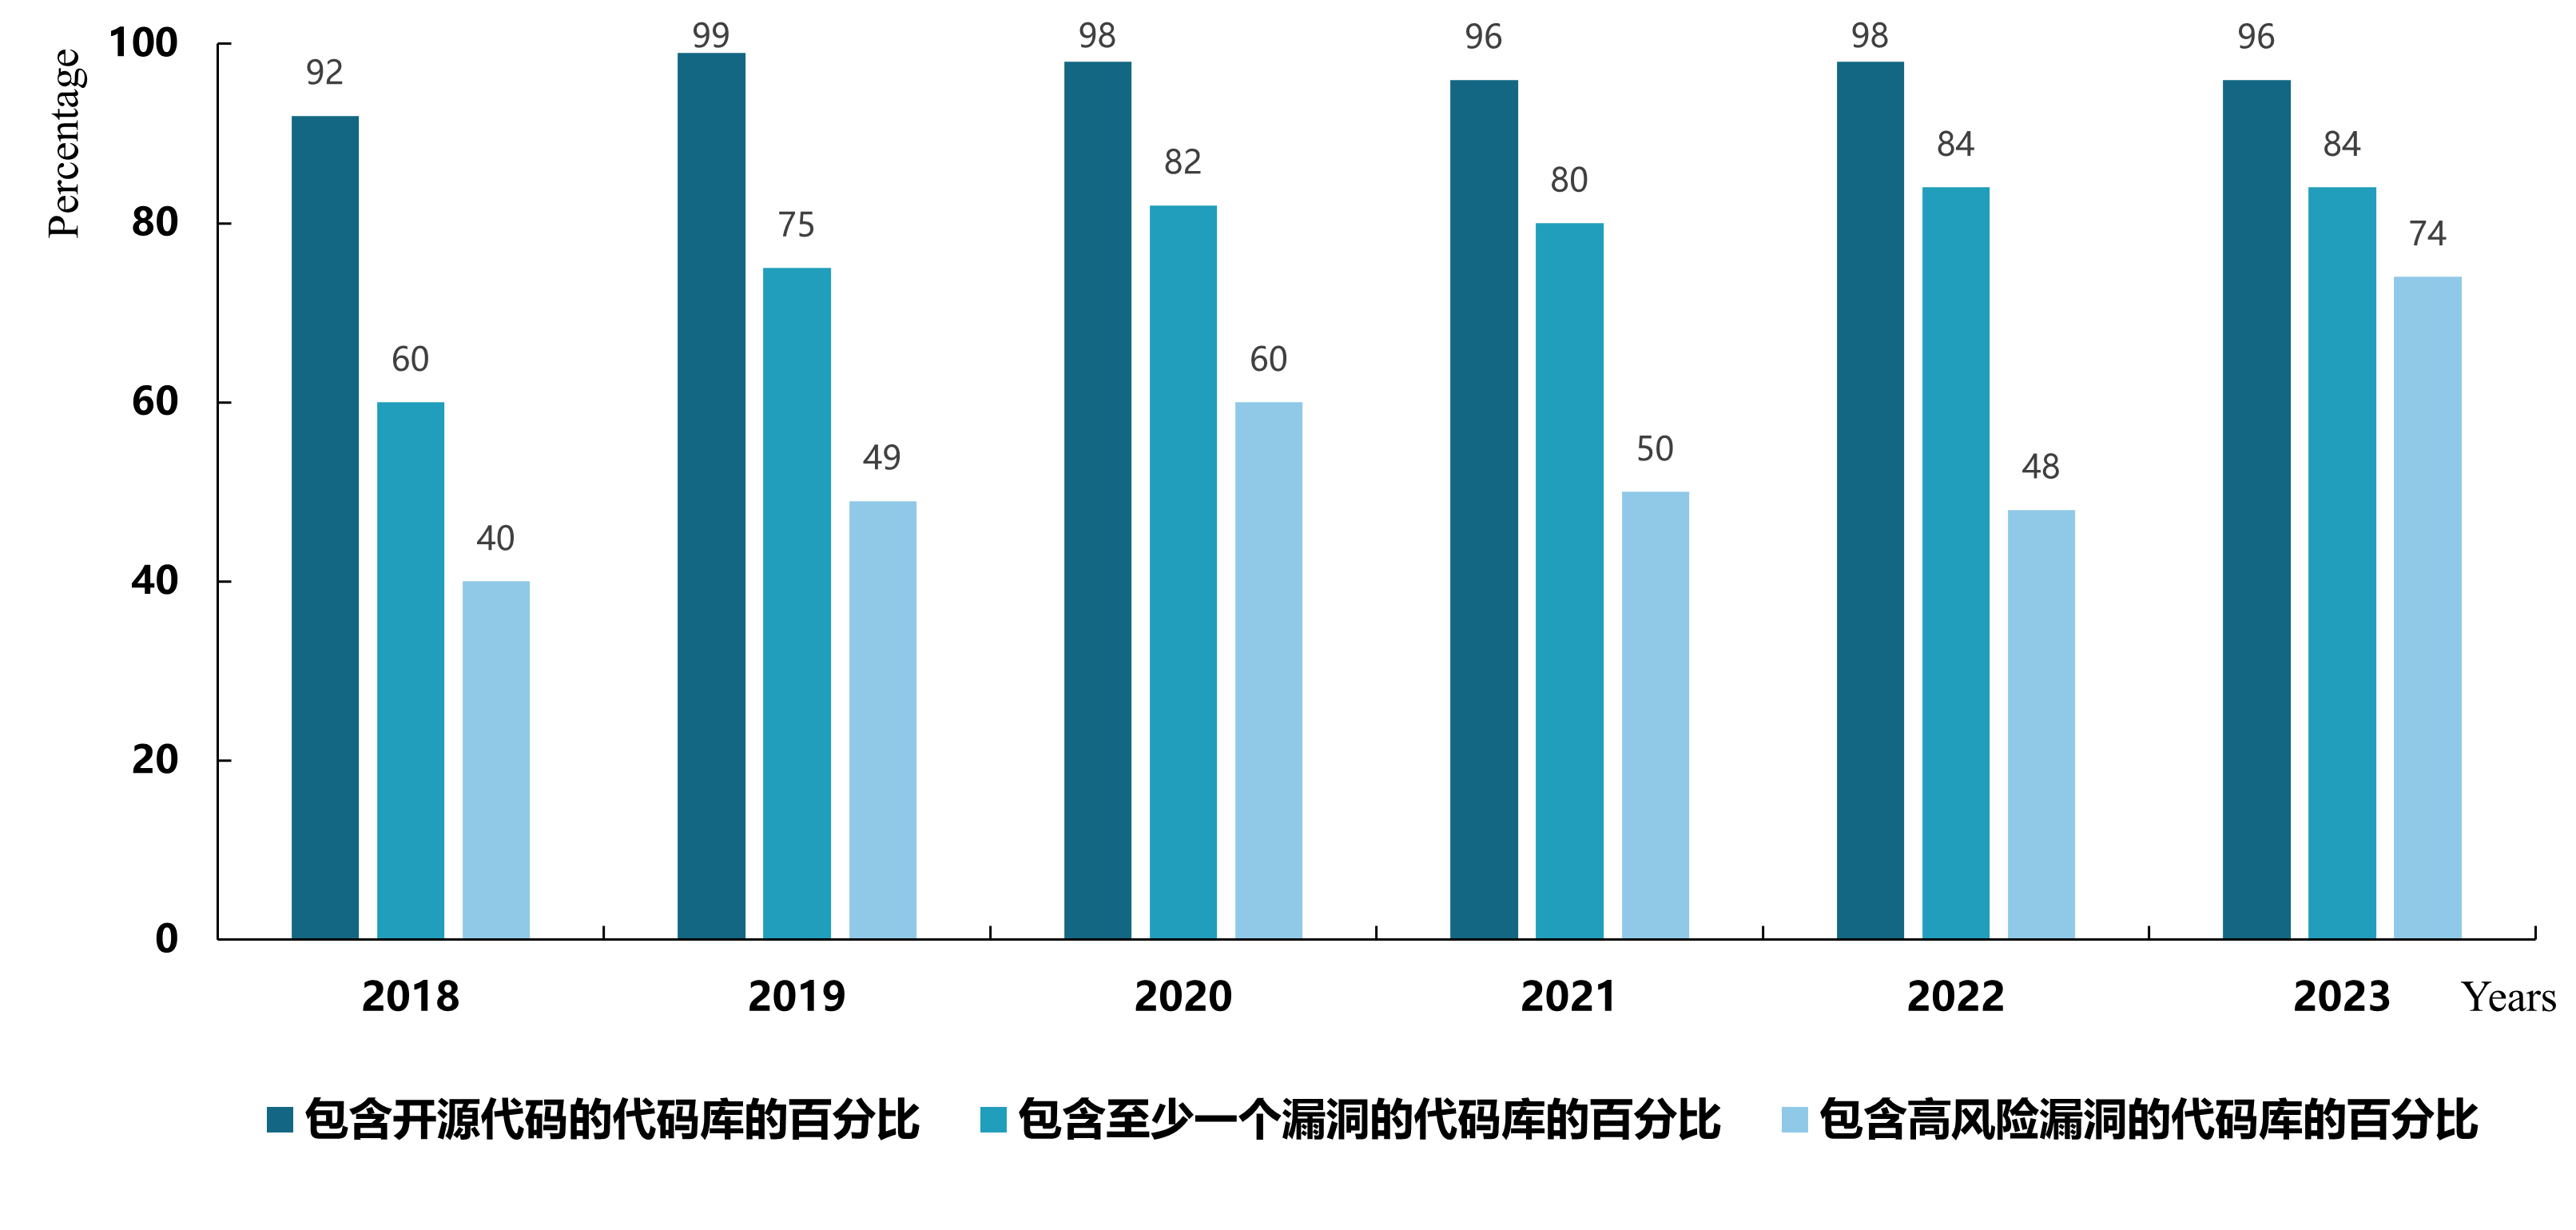
\includegraphics[width=0.95\textwidth]{figures/Proportion}
    \caption{2018-2023年Synopsys审计代码库中的开源代码及漏洞占比示意图}\label{fig:Proportion}
\end{figure}

同时,Synopsys按照行业划分,统计了各行业包含开源代码的占比,其中互联网等相关行业包含开源代码的代码库百分比均为100\%,其余行业占比如图\ref{fig:assembly}所示。此外,经过风险评估的代码库中,14\%包含10年以上的漏洞,漏洞的平均年龄为2.8年,49\%包含24个月内未更新的组件。一旦这些组件出现安全问题,通常会导致软件遭受供应链攻击。据Gartner\cite{Gartner_2022}预测,到2025年,全球45\%的组织将遭受软件供应链攻击,比2021年增加三倍。因此,准确地检测代码克隆对于软件开发和维护至关重要。

\begin{figure}[H]
    \centering
    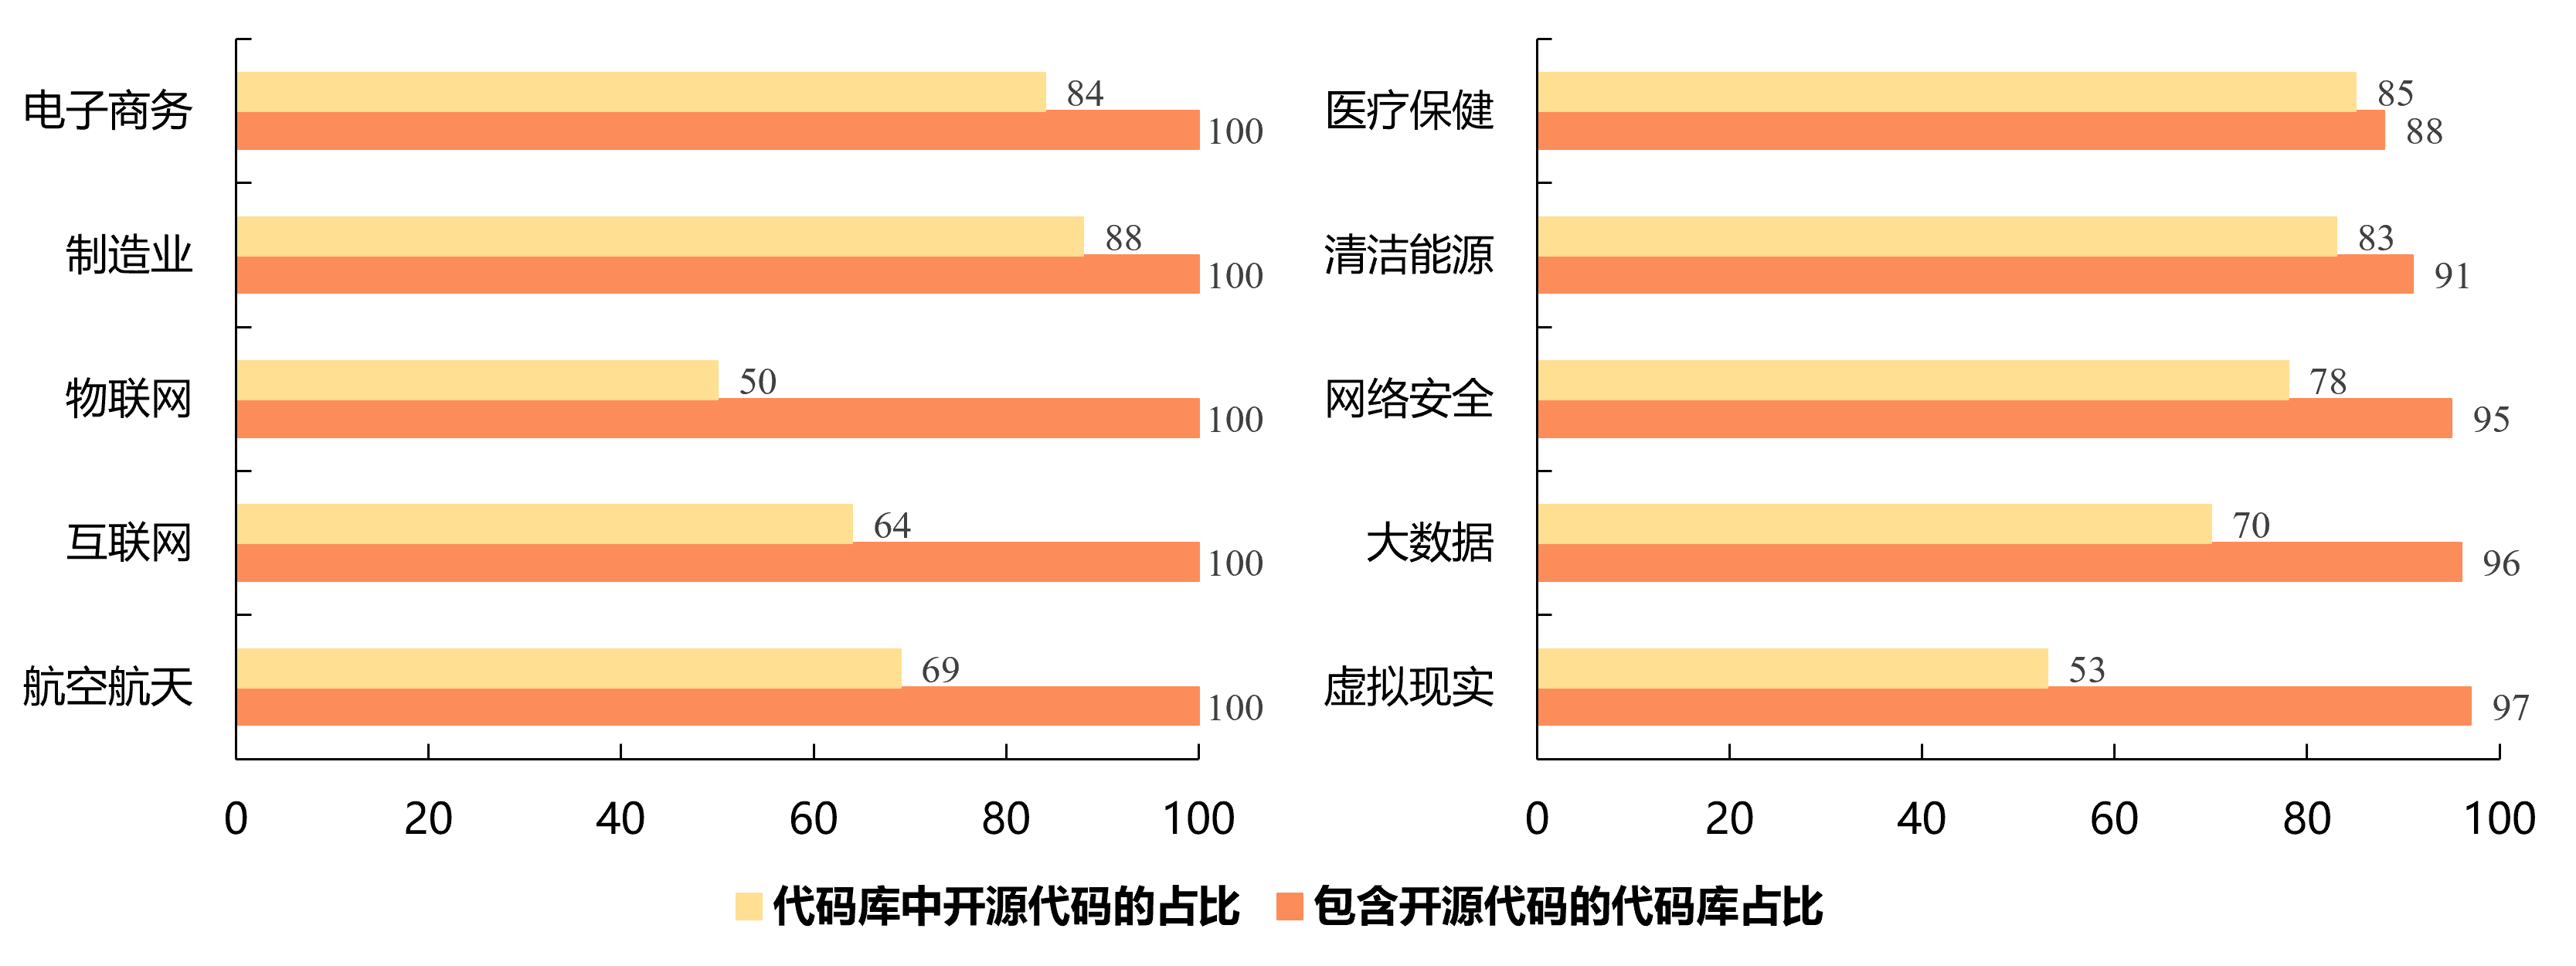
\includegraphics[width=0.95\textwidth]{figures/assembly}
    \caption{2022年Synopsys审计代码库中包含易受攻击组件的百分比示意图}
    \label{fig:assembly}
\end{figure}

早期进行代码克隆检测通常采用人工检查并标注的方法,通过收集整理大量的代码逐行检查语法、语义结构,由人工复查筛选出正确的克隆代码并对其进行标注,由此形成了早期的代码克隆数据样本,例如,2015年Svajlenko\cite{7332459}等三名克隆领域的专家评委花费了216小时通过人工验证方法构造了BigcloneBench数据集,该数据集总数据量达到800万条,其背后的人工花费巨大。这种利用人工的方法检测代码克隆效率低,成本高,并且无法保证准确率\cite{7965429},因此,有研究人员提出代码克隆检测技术,目的在于自动化定位软件系统中的代码克隆,并能够节约成本,减少出错风险\cite{Yang2015ClassificationMF}。

早期代码克隆检测技术通常将代码视为自然语言文本进行处理,通过文本相似性判断代码相似程度;随着编译技术的发展,研究者们将编译原理中的词法分析技术运用到代码克隆检测领域;近年来,基于多维源代码表征学习的代码克隆检测技术引起了学者们广泛的兴趣,有研究人员从代码克隆检测与代码表征学习技术相结合这一方面进行了探索,试图从关键技术点入手,找到合适的结合点,以提高定代码克隆检测技术的效率和智能化程度。


\section{研究现状与趋势}
\label{sec:status}

\subsection{代码克隆检测技术}
\label{subsec:Code clone detection}

代码克隆检测技术,旨在自动化定位软件系统中的代码克隆,节省成本,减少出错风险,从而更好地保证软件质量。目前已有的代码克隆方法大多需要对代码片段进行信息抽取,转换为中间表征,然后根据表征方式的不同,计算不同代码片段之间的相似度,完成克隆检测任务。其具体流程如图\ref{fig:figure1}所示。
\begin{figure}[H]
    \centering
    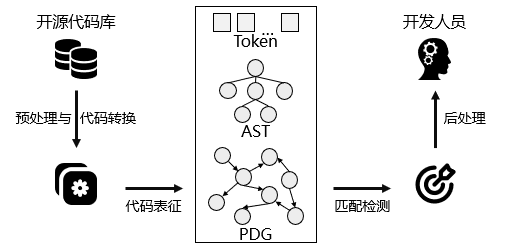
\includegraphics[width=0.95\textwidth]{figures/figure1}
    \caption{代码克隆检测流程}\label{fig:figure1}
\end{figure}

从图\ref{fig:figure1}可以看出一个完整的代码克隆检测过程通常包括预处理与转换、代码表征、匹配检测、后处理几个阶段。具体而言,一般的代码克隆检测从代码预处理与转换开始,首先删除与检测无关的空白行、注释、缩进等元素,并根据检测粒度将源代码划分为单独的片段,比如类、函数等;然后在代码表征步骤,将比较单元转换为词法单元(Token)、抽象语法树(abstract syntax tree,AST)、程序依赖图(Program dependency graph,PDG)等常见的中间表示;在匹配检测阶段,将根据得到不同的中间表示采用相应的匹配算法进行相似度计算,例如抽象语法树的比较通常采用子树匹配算法,程序依赖图的比较则采用子图同构算法。此阶段将代码片段两两对比,以查找相似代码源片段,得到代码克隆对。最后在后处理阶段,通常会通过人工检测或者算法过滤掉错误的代码克隆,并以适当的方式呈现给开发人员提供帮助。

在这些步骤中,代码表征方式决定了匹配检测方法的预处理方式、模型设计、部署方式、运行效率,并影响最终结果\cite{陈秋远2019代码克隆检测研究进展}。比如将源代码表征为文本,其预处理过程主要为去除噪声,如空格、注释等,其比较算法可以利用文本相似的一系列方法,能够检测到语法相似的克隆代码;而如果表征为抽象语法树,则其预处理过程需要解释器的参与,相似比较算法也更多地考虑了结构相似等,能够检测到语法层面相似的代码克隆。由此可见, 代码表征方式是代码克隆检测的关键步骤。


\subsection{代码表征学习}
\label{subsec:Code representation}
表征学习是指学习数据的表示,使其在构建分类器或其他预测因子时更容易提取有用信息\cite{Bengio2013Representation}。代码表征学习是对源代码的语义和语法信息进行表征,得到源代码的特征向量,并将其应用在不同的下游任务上。在代码克隆检测中,代码表征学习可以用来提取代码片段更高层次的抽象特征表示,这些特征表示能够捕捉代码的语法、语义以及结构信息。通过学习到的代码表征,可以更准确地比较和识别不同代码片段之间的相似性,从而实现克隆代码的检测和管理,提高检测的准确性和鲁棒性。因此,代码表征学习为代码克隆检测提供了重要的技术支持。

早在100多年前,基于传统机器学习的数据特征学习就被广泛提出\cite{wiki},主成分分析PCA(Principal Component Analysis)\cite{WOS:000202849800065}、线性判别分析LDA(Linear Discriminant Analysis)\cite{2012THE}都是经典的表征学习方法。随着神经网络的不断发展,基于深度学习的代码表征学习工作能够更有效地提取数据的特征,用于后续的分类或预测。2013年,Y Bengio等人\cite{Bengio2013Representation}发表了关于表征学习的经典综述。2016年,Bengio和 IGoodfellow等人\cite{goodfellow2016deep}合著的《Deep Leanring》一书中为表征学习专著一章。近些年来,代码表征学习方法被用于代码克隆检测、代码推荐、代码剽窃等多个代码分析任务中,取得了一定的成就。根据源代码的抽象层次不同,现阶段代码表征学习工作可以分为基于Token的代码表征、基于树的代码表征、基于图的代码表征、基于语法和语义混合的代码表征四类。

(1)基于Token的代码表征

基于Token的代码表征通常利用词法分析器将代码中的词汇单元(Token)划分出来。这些词汇单元通常包含关键字、数字、标识符等。将代码表示为词汇单元序列之后,对其进行建模,学习代码序列中所包含的有效信息,如功能语义信息、语法结构信息等,最后生成具有丰富代码信息的表征向量,应用于后续的代码克隆检测任务中。

著名的CCFinder\cite{1019480}、CP-Miner\cite{1610609}等经典代码克隆检测工具都是基于Token级的,可以很好地检测完全相同的代码对以及参数化后的代码对克隆问题。其中,CCFinder将源代码中的每一行单独转换为Token序列,根据转化规则对Token进行修改,将类型名、变量名、常量的标识符替换为指定的特殊Token,最后利用后缀树来查找相同的子序列并通过设置阈值来过滤克隆对。CP-Miner增加了Bug检测,该工具的检测速度、检测精度相较于CCFinder有了很大的提高。

Jiang等人\cite{10.1145/1287624.1287634}首先使用神经网络在Token级别进行代码克隆检测,提出CCLearner方法。该方法使用BigCloneBench\cite{7332459}作为训练样本,抽取了其中方法级别的Token序列,将保留字、类型标识符、方法标识符和变量标识符等8种符号表示为8种标记,随后将各种标记类型以及出现的频数作为代码的序列表示,并用于代码克隆检测。

Mikolov等人\cite{pennington-etal-2014-glove}利用Word2vec、GloVe、BERT进行Token的预训练,通过无标注样本训练深度网络结构,使用标注样本进行模型参数微调,从而提升模型性能。其中BERT\cite{devlin-etal-2019-bert}是双向Transformer的编码器,通过遮蔽语言模型和下一句预测2种预训练目标来调整模型参数。

Sajnani等人\cite{7886988}提出了一种基于词袋模型的代码表征方法SourcererCC,使用代码段Token的组成来度量两段代码块中词法粒度上的重复度,从而检测两段代码的相似性。这种方法相对于纯文本的代码表示形式实现了更高层次的代码分析。

Tao等人\cite{9796359}提出了一种跨语言克隆检测模型C4,通过对比学习的思想,采用预先训练的模型CodeBert提取代码特征,并转换为高维代码表示。此外,还通过一个可以有效识别克隆对和非克隆对的约束学习目标来微调C4模型。实验结果表明,C4在准确率、召回率、F1方便显著优于最先进的基线。

上述方法均在Token上进行代码的表征学习,力图充分提取代码中的属性信息。

(2)基于树的代码表征

抽象语法树AST最早由Yourdon等人\cite{10.1145/1499949.1499997}提出,是源代码的抽象语法结构的树状表示,可以有效地表示程序的语法及其结构,利用深度神经网络对抽象语法树进行建模得到其向量表示,根据该特征向量完成代码克隆检测任务,实现基于树的源代码表征。

White等人\cite{White2016DeepLC}提出了一种基于循环神经网络的代码表征方法,该方法将代码分为词汇以及句法两个层次。对于词汇级别的信息,该方法在代码的词汇单元序列上使用RNN神经网络进行建模。而对于代码的句法级别的信息,首先将代码转换为其对应的抽象语法树结构,之后将抽象语法树转换为其对应的满二叉树,最后将满二叉树转换为橄榄树,并在其上使用另一个RNN神经网络进行建模。该方法将这两个特征相结合作为整个程序的特征向量,根据该向量进行代码克隆检测任务。

Mou等人\cite{WOS:000485474201046}提出了一种基于树的卷积神经网络模型TBCNN(Tree-based convolutional neural network)。该模型采用了“连续二叉树”的概念,直接在代码所对应的抽象语法树上进行卷积操作。在卷积操作之后获得了不同数目的AST结构特征向量,由于数目不同不能直接作为神经网络的输入,因此该方法还采用“动态池化”技术,最终将数目不同的特征向量转换为了一个向量。TBCNN是一个通用的代码表征生成模型,所生成的向量能够包含代码片段中特有的代码模式,因而可以应用于不同的代码分析任务中。

Wei等人\cite{10.5555/3172077.3172312}提出了一种基于哈希的代码表征方法CDLH(Clone Detection with Learning to Hash)。该方法使用Word2Vec模型学习标记嵌入以捕获词汇信息,然后训练基于抽象语法树的LSTM模型将这些嵌入组合成一个二进制向量来表示代码片段,最后通过计算哈希码的汉明距离来检测代码克隆。

Zhang等人\cite{8812062}提出了一种基于抽象语法树的神经网络代码表征方法ASTNN(A novel AST-based Neural Network )。该方法将完整的抽象语法树分割为多个语句子树。针对每个语句树,该方法设计了语句编码器用于将语句树转换为对应的语句表征向量,通过使用双向GRU神经网络对语句向量进行建模,对双向GRU层输出的隐含状态向量进行最大池化操作,以获得最显著的代码特征。该方法所生成的代码表征向量被应用于代码克隆检测任务中,在POJ104\cite{WOS:000485474201046}和BigcloneBench\cite{7332459}数据集上取得了当时最好的检测结果。

Yu等人\cite{8813290}提出了一种基于树卷积的代码表征方法TBCCD(Tree-Based Convolution for Clone Detection)。该方法提出了一种三角形卷积核对父节点和子节点卷积,通过自适应的参数编码树中的节点;同时考虑到抽象语法树的词法信息,通过位置相关的编码方式编码Token值,最后基于CNN进行克隆检测。

Ling等人\cite{Ling2022ImproveRF}提出了一种树自动编码器架构TAE。该方法使用无监督学习对大规模数据集的抽象语法树AST进行预训练,然后在下游任务代码克隆检测任务中对训练后的编码器进行微调,实现跨语言代码克隆检测。

Wu等人\cite{10.1145/3551349.3560426}提出了一种基于树的可扩展的语义代码克隆检测器Amain,通过将抽象语法树转换为简单的马尔科夫链,并测量马尔科夫链中所有状态的距离,将距离值送入分类器中训练得到一个代码克隆检测器。

上述方法均在抽象语法树上进行代码的表征学习,力图充分提取代码中的结构信息。

(3)基于图的代码表征

程序依赖图PDG最早由Ferrante J等人\cite{10.1145/24039.24041}提出,是程序的一种图形表示,所含结构信息最多,能够表示程序的控制依赖,数据依赖以及地址依赖等关系,是一种带有标记的有向多重图。通过将程序表示为图的形式使得模型能够更好地理解代码中不同部分之间的依赖关系。

Allamanis等人\cite{Allamanis2017LearningTR}考虑到代码中的长依赖问题,如在代码中变量的定义位置与使用位置之间的距离问题,提出了基于图的代码表征方法,并介绍如何使用GGNN(Gated Graph Neural Networks)训练。首先将代码转换为对应的抽象语法树,之后通过不同的连接规则连接抽象语法树各个节点,获得了包含变量之间依赖关系在内的不同节点之间的关联关系;最后将构建好的代码图数据作为输入,输入到图神经网络中进行表征学习。

Lu等人\cite{Lu2019ProgramCU}提出了一种用于程序分类的图网络模型GGANN(Gated Graph Attention Neural Networks)。该方法从代码中提取数据流与函数调用信息,将其融合到抽象语法树中,从而将代码构建为一个包含丰富信息的图结构表示FDA。在传统的GGNN模型上引入了注意力机制,用于获得图中每个节点的重要程度,进而获得更具有区分度的代码表征向量。

Brockschmidt等人\cite{Brockschmidt2018GenerativeCM}提出了一个生成代码模型,该模型利用部分生成程序的已知语义来指导生成过程。关键思想是在代码的抽象语法树上增加相应的边以构建代码图,之后使用图神经网络对已获得的部分程序的结构和数据流进行建模完成代码表征任务。这种表示有助于更好地指导生成过程的剩余部分。

Ben-Nun等人\cite{10.5555/3327144.3327276}提出了一种与语言以及平台无关的代码表征方法inst2vec。该方法首先使用编译器对代码进行编译,得到代码的中间表示。但由于该中间表示并没有包含代码之中的数据流信息以及控制流信息,因此该方法将数据流和控制流也融合到该中间表示中,进而构建了代码上下文流图,最后在所构建的图上使用循环神经网络进行建模,获得代码的表征向量。该向量在程序分类实验中的准确率取得了当时最好的效果。

Wang等人\cite{9054857}提出了一种称为流增强抽象语法树FA-AST(Flow-Augmented Abstract Syntax Tree)的程序图表示,考虑了仅仅使用代码的抽象语法树进行代码表征建模实际上仍然有代码结构上的缺失这一问题,构建了代码抽象语法树的图形表示FA-AST,通过将抽象语法树各个叶子结点相连构建出适合图神经网络处理的数据,然后应用两种不同类型的图神经网络GNN来检测克隆。

DeFreez等人\cite{10.1145/3236024.3236059}提出了一种学习嵌入方法Fun2Vec,将每个函数映射到连续向量空间中的向量,以便使同义函数的向量非常接近。该方法采用随机游走算法,在程序的过程间控制流图上随机选择部分执行路径,捕获程序的层级结构,每条执行路径转换为一个标签序列,借助Word2Vec方法,把标签映射为连续实值向量,并通过神经网络训练函数的嵌入向量。

Kang等人\cite{Yang2021AGS}提出了一种针对代码补全问题的门控卷积网络模型CC-CCNN。该方法通过从代码表示中获得有效的代码特征,提出了一种分类机制,通过使用已知的父节点对节点的表示进行分类,并在模型中构建训练图。实验结果表明,模型在数据集中最多优于最先进的方法MRR最多9.2\%,ACC最多11.4\%。

上述方法均在图上进行代码的表征学习,力图充分提取代码中的语义信息。

(4)基于语法和语义融合的代码表征

基于语法与语义融合的模型,结合抽象语法树AST、数据流图DFG、控制流图CFG、词法单元Token序列,捕获程序的语法及语义结构信息。其中抽象语法树AST和Token序列反映了语法层面的信息,数据流图DFG、控制流图CFG反映了语义层面的信息。

Tufano等人\cite{Tufano2018DeepLS}采用四种不同的代码表征方法(即标识符Token、抽象语法树AST、字节码和控制流图CFG)进行代码克隆检测,他们利用四种代码表示分别识别代码对的相似度,并计算平均值作为最终的相似度结果。

Saini等人\cite{10.1145/3236024.3236026}提出了一种基于多种度量的代码克隆检测框架Oreo,该方法从程序的源代码中提取了包括被调用的外部方法的数量、变量的数量、语句的数量、循环的数量等24种度量,然后进一步从函数中抽取语义,并使用了基于哈希的方法进一步筛选,最后加入了深度学习的方法,将两个程序向量输入到孪生模型中来判断两个程序之间是否具有克隆关系。

Fang等人\cite{Fang2020FunctionalCC}结合抽象语法树,控制流图和调用图来学习代码特征,融合了语法和语义信息。首先,该方法从源码中分析出方法之间的调用图、每个方法的抽象语法树以及每个方法的控制流图;然后,用调用图找出每个功能的AST集合。通过AST集合抽取功能的语法信息;通过调用图组成每个功能的控制流图;通过控制流图抽取功能的语义信息;最后,将抽取出来的语义信息送入前馈神经网络得到分类结果。

Hua等人\cite{Hua2020FCCAHC}提出了一种使用注意力机制的功能代码克隆检测器FCCA(Functional code clone detector using attention),结合标记、抽象语法树和控制流图三种方式实现检测目标。该方法通过保留多个代码特征,包括非结构化(顺序令牌形式的代码)和结构化(抽象语法树和控制流图形式的代码)信息,在混合代码表示的基础上进行代码克隆检测。将多个代码特征融合到混合表示中,该混合表示配备有注意力机制,有助于最终检测精度的重要代码部分和特征。

Dong等人\cite{9148302}提出了一种基于Token和AST的代码表征方式,提取数量特征如AST中的AST树的高度、节点数以及标记中操作数的个数、字符串的个数等作为神经网络的输入进行检测。

Feng等\cite{Feng2020CodeBERTAP}提出了一种多模态的预训练模型,利用不同模态的信息互补作用,有效提升了模型的整体表征能力。CodeBERT基于文档和代码,在自然语言和程序语言双模态下,利用BERT进行预训练,提取自然语言和程序语言之间的语义连接,为下游任务提供通用表示向量。

Duan等人\cite{WOS:000680742600067}提出了一种无监督的程序代码表示学习技术DEEPBINDIFF,依靠代码语义信息和程序控制流信息生成基本块嵌入,并且采用k-HOP贪婪匹配算法,利用基本块嵌入发现最优的相似性结果。通过大量二进制文件和真实的OpenSSL漏洞对原型进行评估,结果表明DEEPBINDIFF相比于最先进的工具,跨版本和交叉优化级别都更优。

Wu等人\cite{10.1145/3324884.3416562}提出了一种基于序列和基于图的软件功能克隆检测方法SCDetector。针对给定的方法源代码,首先生成控制流图,然后应用社交网络中心性分析将图转换为某些语义标记(即具有图细节的标记)。最后,这些语义标记被馈送到Siamese网络中,以训练模型并使用它来检测代码克隆对。

总体而言,代码克隆检测是提高软件开发质量的重要手段,如何对代码进行合适的表征是代码克隆检测的关键问题\cite{JSYJ20240123005}。代码表征学习决定了对源代码信息抽取程度的上限,决定了检测技术的预处理方法、模型设计、部署方式、运行效率,并会影响最终结果。面向代码克隆检测这一下游任务,基于Token的方法将代码视为文本,保留了源代码本身存在的噪声,缺少代码的语义、结构信息;基于树的方法在一定程度上提取了代码的结构信心,但在转换AST的过程中会丢失部分信息,并且存在信息冗余;基于图的方法保留了语法和语义信息,但在生成图的过程中需要付出较高代价。以上单个维度的代码表征方法各有利弊,但总体对代码信息利用不充分,因此,研究人员一方面通过对源代码进行充分利用,提出多维源代码表征方法,从而提高代码克隆检测能力;另一方面,通过研究更先进的算法来提高表征模型的适应性和泛化能力,也是目前重要的发展趋势。

\section{研究内容}
\label{sec:Content}
本文主要围绕如何将源代码表征学习技术应用到代码克隆检测领域的问题,通过不同维度对程序进行表征学习,并基于学习得到的语义特征进行克隆对的判定,充分发挥代码表征学习技术检测代码克隆的能力。针对现有代码表征学习方法存在的对代码结构信息和语义信息利用不充分的问题,本文提出面向代码克隆检测的多维源代码表征学习方法RLCCD ,旨在通过构建三个不同维度的代码表征模型,将源代码的语义信息表示为稠密低维实值向量,以在低维空间中高效计算实体和关系的语义联系,并通过特征融合得到多维特征,实现对代码信息的充分利用,以更加全面准确与智能化的方式提高代码克隆测试效率。

本文的主要工作包括:

(1)提出面向代码克隆检测的多维源代码表征学习方法RLCCD 

本文提出了一种面向代码克隆检测的多维源代码表征学习方法RLCCD,该框架主要针对代码表征提出三个关键技术点,从Token序列、抽象语法树AST、程序依赖图PDG三种不同维度对代码特征表示进行优化,分别形成了基于预训练辅助模型的Token表征学习、基于子树划分的抽象语法树表征学习、基于图过滤的程序依赖图表征学习三种方法,然后通过特征融合将三种维度特征整合为一个多维特征,实现对代码信息的充分利用,以更加全面准确与智能化的方式提高代码克隆测试效率。 

(2)基于预训练辅助模型的Token表征学习

针对目前现有的基于Token的表征学习方法通常将代码表示为词汇单元,为了后续生成表征向量通常会将词汇单元规范化,丢失部分语法信息,出现在词汇表中不存在Token的难题,提出了一种基于预训练辅助模型的Token表征学习方法。该方法在模型训练之前,通过选取预训练辅助模型从代码语料库中学习基本单元的语法语义信息,以及这些单元之间的联系,最终给出一份单词-向量形式的词汇表,从而减少出现集外词问题的概率。在POJ104数据集上的消融实验评估表明,预训练辅助模型方法能够提高代码克隆检测准确率。

(3)基于子树划分的抽象语法树表征学习

针对现有的基于树的表征学习方法通常将抽象语法树转换为完整二叉树,可能破坏源代码原有语法结构,增加AST高度,丢失长期上下文信息,削弱了神经网络模型捕捉更真实和复杂语义能力,导致梯度消失的难题,提出了一种基于子树划分的抽象语法树表征学习方法。该方法将每个大型的AST分割成小语句树序列,并通过捕获语句的词法和句法知识将每一个语句树都编码成一个向量,在得到一个语句向量序列后,将语句向量序列输入树卷积神经网络中生成代码片段的结构向量表示。在POJ104数据集上的消融实验评估表明,子树划分方法能够有效提取结构特征,提高代码克隆检测准确率。

(4)基于图过滤的程序依赖图表征学习

针对现有的基于图的表征学习方法通常将程序表征为有向多重图,继而采用图匹配算法将图中的控制流和数据流编码为一个紧凑的语义特征矩阵,矩阵中每个元素都是高维系数特征向量,所消耗的时间、空间开销巨大的难题,提出了一种基于图过滤的程序依赖图表征学习方法。该方法通过收集PDG的简单特征来过滤掉明显不可能为克隆的PDG对。具体的,根据PDG的节点个数、控制边数、执行边数、数据边数、声明节点数、函数调用数、传入参数、传出参数等代表特征进行过滤,从而减少候选PDG对规模。在POJ104数据集上的消融实验评估表明,图过滤方法能够有效减少时间、空间开销,提高代码克隆检测准确率。

(5)特征融合及实验验证

针对单个维度对代码信息利用不充分的问题,提出了基于多模态学习的特征融合方法,通过融合多个代码特征,包括非结构化(顺序Token形式的代码)和结构化(抽象语法树和程序依赖图形式的代码)信息,从多维数据中学到更好的特征表示。同时,选取了代码克隆检测领域常见的基准集POJ104进行实验验证,并与现有开源的SourcererCC\cite{7886988}、ASTNN\cite{8812062}、SCDetector\cite{10.1145/3324884.3416562}方法进行比较,主要通过精确度(Precision)、召回率(Recall)、F1值三个指标评价实验结果,实验结果验证了RLCCD的可行性和有效性。

\section{论文结构}
\label{sec:Summary1}
本文总共分为六章,各章节的主要介绍内容如下,组织架构图如图\ref{fig:Structure}所示:

\begin{figure}[H]
    \centering
    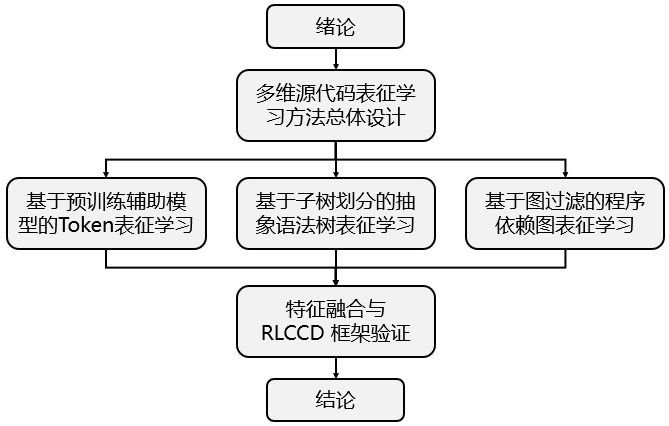
\includegraphics[width=0.95\textwidth]{figures/Structure}
    \caption{论文组织结构}\label{fig:Structure}
\end{figure}

\textbf{第1章} \quad 绪论部分首先对本文的研究背景与意义进行了阐述,之后对代码克隆检测技术和代码表征学习技术的研究现状与趋势进行了分析总结,进而提出本文的主要研究内容,最后介绍了全文的组织结构。

\textbf{第2章}  \quad 分析了代码表征学习领域的关键技术挑战,基于此,提出了本文的面向代码克隆检测的多维源代码表征学习方法RLCCD,并对该方法的整体框架进行了介绍,进而根据所提框架简要论述了本文研究的关键技术,即基于预训练辅助模型的Token表征学习方法、基于子树划分的抽象语法树表征学习方法、基于图过滤的程序依赖图表征学习方法,最后进行本章小结。

\textbf{第3章}  \quad 介绍基于预训练辅助模型的Token表征学习方法的设计与实现。首先,分析其研究动机,即目前Token表征学习面临的集外词问题,继而提出基于预训练辅助模型的方法设计,详细介绍该方法的设计思路和具体实现,最后,通过消融实验验证,评估本章提出的预训练辅助模型的有效性。

\textbf{第4章}  \quad 介绍基于子树划分的抽象语法树表征学习方法设计与实现。首先,分析其研究动机,即目前抽象语法树表征学习面临的梯度消失问题,继而提出基于子树划分的方法设计,详细介绍该方法的设计思路和具体实现,最后,对该方法的有效性进行消融实验验证。

\textbf{第5章}  \quad 介绍基于图过滤的程序依赖图表征学习方法设计与实现。首先,分析其研究动机,即目前图表征学习面临的规模开销问题,继而提出基于图过滤机制的方法设计,详细介绍该方法的设计思路和具体实现,并给出了针对该方法有效性的消融实验验证。

\textbf{第6章}  \quad 介绍特征融合及本文研究框架RLCCD的实验验证。首先,针对特征融合的方法设计与具体实现进行了介绍。接着,对RLCCD框架的有效性进行了评估,通过与现有开源技术SourcererCC\cite{7886988}、ASTNN\cite{8812062}、SCDetector\cite{10.1145/3324884.3416562}进行实验对比,验证RLCCD方法的有效性。

\textbf{结论}  \quad 首先对全文的研究工作进行了总结,并讨论本文的主要贡献与创新之处,最后对下一步可开展的工作提出展望。